\documentclass[12pt]{book}

\usepackage{amsmath, amsthm, mathtools, amssymb}
\usepackage{thmtools}

\usepackage{enumitem}
\usepackage{parskip}
\usepackage{pdfpages}
\usepackage{float}
\usepackage{tikz}
\usepackage{graphicx}
\usepackage[utf8]{inputenc}

\usetikzlibrary{automata, arrows.meta, positioning}

\newcommand{\HRule}[1]{\rule{\linewidth}{#1}}

\declaretheoremstyle[name=Theorem,]{thmsty}
\declaretheorem[style=thmsty,numberwithin=section]{theorem}

\declaretheoremstyle[name=Definition,]{prosty}
\declaretheorem[style=prosty,numberlike=theorem]{definition}

\newtheorem{lemma}{Lemma}[section]

\newcommand*{\successor}{%
    \stackrel{\scriptscriptstyle\!+\!}\longrightarrow%
}

\newcommand*{\lsuccessor}{%
    \stackrel{\scriptscriptstyle\!+\!}\longleftarrow%
}

\newcommand*{\too}{%
    \stackrel{\scriptscriptstyle\!*\!}\longrightarrow%
}

\newcommand*{\ltoo}{%
    \stackrel{\scriptscriptstyle\!*\!}\longleftarrow%
}

\makeatletter
\newcommand{\chapterauthor}[1]{%
  {\parindent0pt\vspace*{-25pt}%
  \linespread{1.1}\large\scshape#1%
  \par\nobreak\vspace*{35pt}}
  \@afterheading%
}
\makeatother

\begin{document}

\title{Lecture Notes}
\maketitle
\newpage

\tableofcontents

\newpage
\chapter{Lecture 2}

\subsection{Abstract Reduction System}
An abstract reduction system is a binary relation $\rightarrow$ over a set of elements $A$.

\subsection{Other Relations defined on $\protect\overrightarrow{A}$}
\begin{description}[labelsep=4em, align=left, labelwidth=2in]

\item[Identity] $\overrightarrow{A^0} = \{(a, a): a \in A\}$

\item[Reflexive Closure] $\overrightarrow{A^=} = \overrightarrow{A} \cup \overrightarrow{A^0}$

\item[Inverse] $\overrightarrow{A^{-1}} = \{(b, a): a \xrightarrow[A]{} b\}$

\item[Transitive Closure] $\overrightarrow{A^+} = \bigcup\limits_{i \, > \, 0} \overrightarrow{A^i}$

\item[Reflexive Transitive Closure] $\overrightarrow{A^*} = \overrightarrow{A^+} \cup \overrightarrow{A^0}$

\item[Symmetric closure] $\overrightarrow{A^\leftrightarrow} = \overrightarrow{A} \cup \overrightarrow{A^{-1}}$

\end{description}

\vspace{2em}

\textbf{Note:} Pay attention to the order of terms in the name of the relations. For example, the transitive symmetric closure isn't necessarily the same as the symmetric transitive closure. Consider the following relation graph to demonstrate this.

\vspace{2em}

\begin{figure}[!h]
\centering
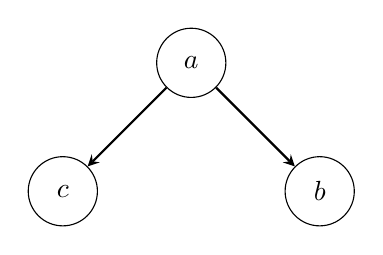
\begin{tikzpicture}
	\node (a) [state] {$a$};
	\node (b) [state, below right = of a] {$b$};
	\node (c) [state, below left = of a] {$c$};
	
	\path [-stealth, thick]
		(a) edge node {} (b)
		(a) edge node {} (c);
		
\end{tikzpicture}
\end{figure}

\begin{align*}
{(A^\leftrightarrow)}^* &= \{(a, a), (a, b), (a, c), (b, a), (b, b), (b, c), (c, a), (c, b), (c, c)\}\\ 
{({A^*})}^\leftrightarrow &= \{(a, b), (a, c), (b, a), (c, a)\}
\end{align*}

\newpage
\subsection{Terminology}

\subsubsection{Describing the elements and their relations}

\begin{itemize}
\item $x$ is reducible if $\exists \, x'$ such that $x \xrightarrow[A]{} x'$.

\item $\theta: F \rightarrow E$ is called an \textbf{invariant} if $\forall x \in A, \theta(x) = \theta(F(x))$. For example, for the run $x_0 \xrightarrow[F]{} x_1 \xrightarrow[F]{} x_2 \xrightarrow[F]{} \cdots$, it must hold that $\theta(x_0) = \theta(x_1) = \theta(x_2) = \cdots$.

\item $x$ is in \textbf{normal form} if it is not reducible.

\item $x$ \textbf{simplifies to} $x'$ in $A$ iff $x \xrightarrow[A^*]{} x'$.

\item $x'$ is a normal form of $x$ in $A$ if: 
\begin{itemize}
\item $x'$ is in normal form
\item $x$ simplifies to $x'$
\end{itemize}

\item $x$ has a normal form in $A$ if $\exists \, x' \in A$ such that $x'$ is a normal form of $x$.

\item $x'$ is an \textbf{immediate successor} of $x$ if $x \xrightarrow[A]{} x'$.

\item $x'$ is a \textbf{proper successor} of $x$ if $x \xrightarrow[A^+]{} x'$.

\item $x'$ is a \textbf{successor} of $x$ if $x \xrightarrow[A^*]{} x'$.

\item Two elements $a$ and $b$ in $A$ are \textbf{joinable} if $\exists \, c \in A$ such that $a \xrightarrow[A^*]{} c$ and $b \xrightarrow[A^*]{} c$. This is denoted as $a \downarrow b$.

\item $a$ and $b$ are \textbf{connected} in $A$ if $a \xrightarrow[{(A^\leftrightarrow)}^*]{} b$

\end{itemize}

\subsubsection{Describing the system as a whole}

\begin{itemize}

\item $\overrightarrow{A}$ is terminating if there is no infinite run: $a_0 \rightarrow a_1 \rightarrow \cdots$.

\begin{figure}[htbp]
\centering
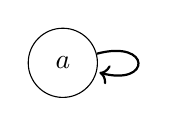
\begin{tikzpicture}
	\node (a) [state] {$a$};
	
	\path [-stealth, thick]
		(a) edge [loop right] node {} (a);
		
\end{tikzpicture}
\caption{A non-terminating relation graph}
\end{figure}

\item $\overrightarrow{A}$ is normalising if every element has a normal form.

\begin{figure}[htbp]
\centering
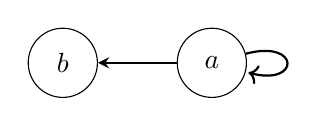
\begin{tikzpicture}
	\node (a) [state] {$a$};
	\node (b) [state, left = of a] {$b$};
	
	\path [-stealth, thick]
		(a) edge [loop right] node {} (a)
		(a) edge node {} (b);
		
\end{tikzpicture}
\caption{A normalising, non-terminating relation graph}
\end{figure}

\item $\overrightarrow{A}$ is confluent if $\forall a, b, c \in A$ such that $a \xrightarrow[A^*]{} b, a \xrightarrow[A^*]{} c$, it must hold that $b \downarrow c$.

\begin{figure}[htbp]
\centering
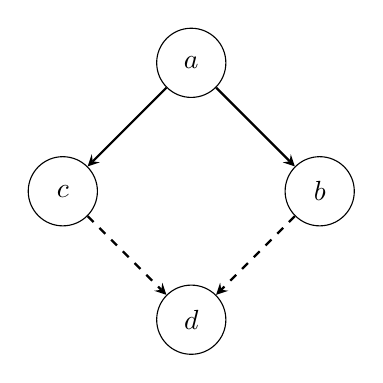
\begin{tikzpicture}
	\node (a) [state] {$a$};
	\node (b) [state, below right = of a] {$b$};
	\node (c) [state, below left = of a] {$c$};
	\node (d) [state, below right = of c] {$d$};
	
	\path [-stealth, thick]
		(a) edge node {} (b)
		(a) edge node {} (c)
		(b) edge [dashed] node {} (d)
		(c) edge [dashed] node {} (d);
		
\end{tikzpicture}
\caption{A visual representation of confluence}
\end{figure}

\end{itemize}

\newpage
\chapter{Lecture 3}
\chapterauthor{Dheeraja Rajreddygari}

\subsection{Properties of abstract reduction systems}

In this lecture, we explore some properties of abstract reduction systems and look at the relationships between them.

\begin{definition}
    An abstract reduction system $( A, \xrightarrow[A]{} )$ is said to be \textbf{Church-Rosser} if $$\forall x, y \in A, \quad x \xleftrightarrow[A]{*} y \implies x \downarrow_A y$$
\end{definition}

Consider abstract reduction systems $A$ and $B$ as shown in the figure below. System $A$ is not Church-Rosser, since $a \xleftrightarrow[A]{*} b$ but $a$ and $b$ are not joinable. System $B$ is a simple example of a Church-Rosser system.

\begin{figure}[htbp]
    \center
    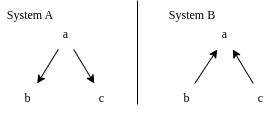
\includegraphics[scale=0.8]{images/lecture1/CR.png}
    \caption{Examples of abstract reduction systems}
\end{figure}


\begin{definition}
    An abstract reduction system $( A, \xrightarrow[A]{} )$ is said to be \textbf{Confluent} if $$\forall a, b, c \in A, \quad a \xrightarrow[A]{*} b \text{ and }  a \xrightarrow[A]{*} c \implies b \downarrow_A c$$
\end{definition}

\begin{definition}
    An abstract reduction system $( A, \xrightarrow[A]{} )$ is said to be \textbf{Semi-confluent} if $$\forall a, b, c \in A, \quad a \xrightarrow[A]{} b \text{ and }  a \xrightarrow[A]{*} c \implies b \downarrow_A c$$
\end{definition}

\begin{theorem}
    For an abstract reduction system, \textbf{Church-Rosser, Confluence and Semi-confluence are equivalent}.
\end{theorem}

\textbf{Proof:} We will prove this theorem in the following three stages. Clearly, the three of them combined result in the theorem stated above.
\begin{enumerate}
    \item $\text{Church-Rosser} \implies \text{Confluence}$
    \item $\text{Confluence} \implies \text{Semi-confluence}$
    \item $\text{Semi-confluence} \implies \text{Church-Rosser}$
\end{enumerate}

First, we will prove that \textbf{if a system is Church-Rosser, it is confluent}. Let $(A, \xrightarrow[A]{})$ be an abstract reduction system that is Church-Rosser. \\
Let $a, b, c \in A : a \xrightarrow[A]{*} b \text{ and } a \xrightarrow[A]{*} c$ \\
By definition, $b \xleftrightarrow[A]{*} c$ \\
Since A is Church-Rosser, $b \xleftrightarrow[A]{*} c \implies b \downarrow_A c$ \\
i.e. $ a \xrightarrow[A]{*} b \text{ and } a \xrightarrow[A]{*} c \implies b \downarrow_A c$, proving that A is confluent


Next, we will prove that \textbf{if a system is Confluent, it is also semi-confluent}. Let $(A, \xrightarrow[A]{})$ be a confluent abstract reduction system. \\
Let $a, b, c \in A : a \xrightarrow[A]{} b \text{ and } a \xrightarrow[A]{*} c$ \\
Since $A \subseteq A^*$, $a \xrightarrow[A]{} b \implies a \xrightarrow[A]{*} b$ \\
Since A is confluent, $a \xrightarrow[A]{*} b \text{ and } a \xrightarrow[A]{*} c \implies b \downarrow_A c$ \\
i.e. $ a \xrightarrow[A]{} b \text{ and } a \xrightarrow[A]{*} c \implies b \downarrow_A c$, proving that A is semi-confluent

Finally, we will prove that \textbf{if a system is semi-confluent, it is also Church-Rosser}. Let $(A, \xrightarrow[A]{})$ be a semi-confluent abstract reduction system. \\
Let $a, b \in A : a \xleftrightarrow[A]{*} b$ \\
Let $p$ be the shortest path connecting $a$ and $b$ in $A^{\leftrightarrow ^*}$. We will use induction on $|p|$ to prove that $a$ and $b$ are joinable. \\
\textbf{Base case:} For $p=0$, we have $a=b$ which makes them trivially joinable. \\
\textbf{Induction step:} Let it be true that if the shortest path connecting $a$ and $b$ in $A^{\leftrightarrow ^*}$ is $|p|$, then $a$ and $b$ are joinable in $A$. We will prove that this is also true for $|p|+1$.

Let $a, b' \in A$ such that the shortest path connecting them in $A^{\leftrightarrow ^*}$ is of length $|p|+1$. Then, $\exists b \in A :$ the shortest path connecting $a$ and $b$ in $A^{\leftrightarrow ^*}$ is $|p|$ and $b \xleftrightarrow[A]{} b'$. Since our induction hypothesis holds true for $|p|$, $a$ and $b$ are joinable (they both reduce to some $c \in A$).


\begin{figure}[htbp]
    \center
    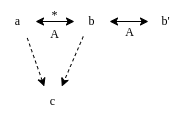
\includegraphics[scale=0.8]{images/lecture1/induction1.png}
    \caption{Abstract reduction system representing the induction step}
\end{figure}
We now have 2 cases. 

\textbf{Case 1:} $b \xleftarrow[A]{} b'$ 

\begin{figure}[htbp]
    \center
    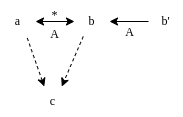
\includegraphics[scale=0.8]{images/lecture1/induction2.png}
    \caption{Abstract reduction system in case 1}
\end{figure}
$b' \xrightarrow[A]{} b \xrightarrow[A]{*} c$. Therefore, $a \downarrow _A b'$. 

\textbf{Case 2:} $b \xrightarrow[A]{} b'$

\begin{figure}[htbp]
    \center
    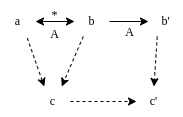
\includegraphics[scale=0.8]{images/lecture1/induction3.png}
    \caption{Abstract reduction system in case 2}
\end{figure}
Here we have $b \xrightarrow[A]{} b'$ and $b \xleftrightarrow[A]{*} c$. Since $A$ is semi-conflient, $b'$ and $c$ must be joinable. That is, $\exists c' \in A : b' \xrightarrow[A]{*} c' \text{ and } c \xrightarrow[A]{*} c'$.  Since $a \xrightarrow[A]{*} c \xrightarrow[A]{*} c'$, we have $a \xrightarrow[A]{*} c'$. Hence, $a \downarrow _A b'$


In either case, we have shown that $a \downarrow _A b'$, which completes our induction. We have proven that $a \xleftrightarrow[A]{*} b \implies a \downarrow_A b$, which means A is also Church-Rosser.

This completes our proof that Church-Rosser, Confluence and Semi-confluence are equivalent properties of an abstract reduction system. While it may seem redundant to have multiple terms to refer to the same thing, they each give us a different perspective of looking at the same property which can prove to be helpful.


\subsection{Address space}
Data structures provide a way to organize and address data. For a data structure, a valid set of addresses form its address space. This is \textbf{not} a formal definition of address spaces and is only meant to give a broad idea. We will look at an example below to illustrate one way of addressing a binary tree. Let us consider the following addressing of a binary tree: each edge is labelled $1$ or $2$ depending on whether it leads to the left or right descendant of a node; the address of each node is obrained by appending the label of the edge leading into it to the address of its parent, with the root being $\epsilon$. Look at the figure below to bettter understand this.
\begin{figure}[htbp]
    \center
    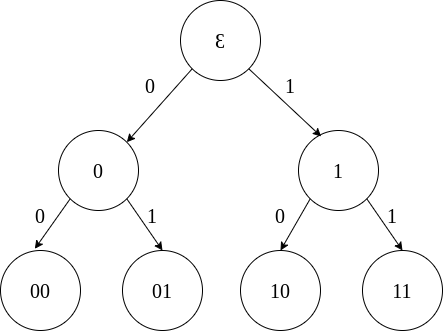
\includegraphics[scale=0.4]{images/lecture1/address.png}
    \caption{Addressing a binary tree}
\end{figure}

The address space for this binary tree would be the set $S = \{\epsilon, 0, 00, 01, 1, 10, 11 \}$. The set $S_1 = \{ \epsilon, 0, 00, 01, 1 \}$ would also be a valid address space for some binary tree but the set $S_2 = \{ 0, 00, 1 \}$ would not, since it does not contain $\epsilon$, the address of the root.

\newpage
\section{Lecture 4}
\subsection{N-Arity}
$\bar{Z_{n}} = [1...n]$

\subsubsection{}An n-ary address space A is a subset of $\Bar{Z^{*}_{n}}$ that is prefix closed if $q: A$ and $p$ is a prefix of q, then $p: A$.\\

Example:
\begin{figure}[htbp]
    \center
    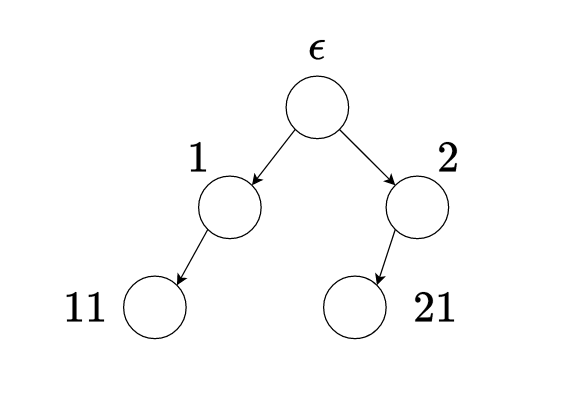
\includegraphics[scale=0.8]{images/popl-4-1.png}
    \caption{}
\end{figure}

$A = {\epsilon, 1, 2, 11, 21}$
\subsubsection{}
Let A be an n-ary address space and let $p:A$ .
\begin{gather}
    A@p = \{q: \bar{Z_{n}^{*}}\  \vert\  pq: A\}  \xrightarrow{} \text{Address space of A relative to p}
\end{gather}

e.g.
\indent $A@2 = \{\epsilon, 1\}$

\subsubsection{}
Context at p (excluding p)
\begin{gather}
    C_{ex}(A, p) = A\backslash pA@p\\
    \xrightarrow{} \text{concatenating p with each address (in subtree) relative to p}
\end{gather}

Context at p (including p)
\begin{gather}
    C_{in}(A, p) = C_{ex}(A,p) \cup \{p\}
\end{gather}
\begin{figure}[htbp]
    \center
    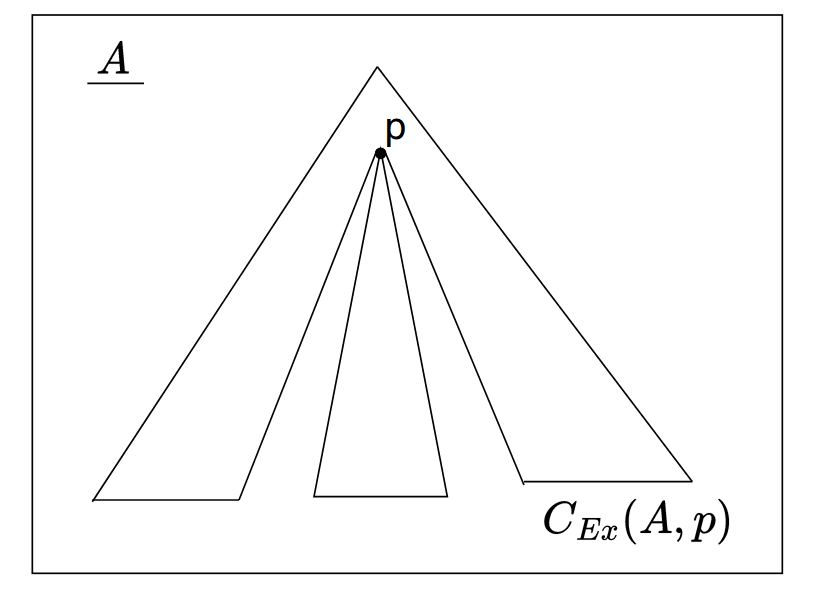
\includegraphics[scale=0.5]{images/popl-4-2.png}
    \caption{}
\end{figure}

\subsection{Terms, Subtrees, Tree Contex}
\subsubsection{}
Let A be an address space. A term is a map $t:A\xrightarrow{}v$ where $V$ is a set of values.

Example:
\begin{gather}
    V = \mathcal{N}, A = \{\epsilon, 1, 2\}\\
    t: \{\epsilon\xrightarrow{}5, 1\xrightarrow{}7, 2\xrightarrow{}7\}
\end{gather}

\begin{figure}[htbp]
    \center
    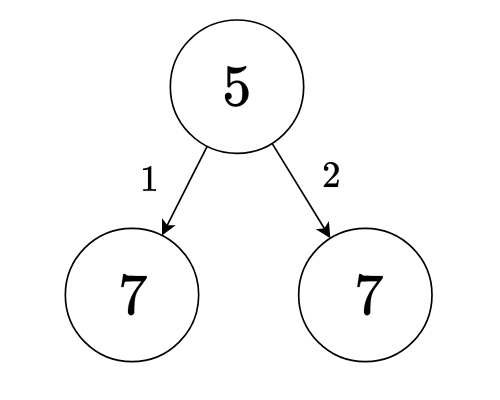
\includegraphics[scale=0.6]{images/popl-4-3.png}
    \caption{}
\end{figure}

\subsubsection{}
Let $t:A\xrightarrow{v}$ be a tree and let $p:A$
\begin{gather}
    C_{ex}(t,p) = df = t \vert_{C_{ex}(A,p}
\end{gather}

\subsubsection{}
Let $\Sigma_{s}$ be a set of symbols.\\
Let $\alpha: \Sigma_{s} \xrightarrow{ \mathcal{N}}$ denote the arity map of $\Sigma_{s}$.\\

Example,\\
\begin{gather}
    \Sigma_{s} = \{f,a,b\}
    \alpha_{s}: \{f\xrightarrow{}2, a\xrightarrow{}0, b\xrightarrow{}0\}\\
    \implies f(a,b) \checkmark \ \ \ \ a \checkmark \ \ \ \ b \checkmark \ \ \ \ f(a) \times
\end{gather}

\subsubsection{}
A term is $(A,\Sigma_{s}, \alpha, t: A\xrightarrow{} \Sigma_{s})$\\
s.t.
\begin{enumerate}
    \item A is a prefix-closed language over $\mathcal{N}_{+}$
    \item $\forall p: A$, if $t_{p}=S$ and $\alpha(S)=n$\\
    then $p1,..., p\alpha(S): A$ \ \ \ \ \  \ \ \ 
    $\forall i: 1 \leq i \leq \alpha(S), pi: A, \forall i: \mathcal{N}_{+}\backslash[1,...,\alpha(S)]pi\notin A$
\end{enumerate}
\newpage

\newpage
\chapter{Lecture 5}
\chapterauthor{Bharat Sahlot}

\subsection{Terms}

\paragraph{ARS} Abstract Reduction System

\paragraph{Terminating ARS} An ARS is terminating \emph{iff.} it has no infinite runs.

\subsection{Well Founded Induction(WFI)}

This is property of an abstract reduction system. A system having this property implies that,

$$
\forall x \in A. \left( \forall y \in A. \ x \successor y \implies P(y) \right) \implies P(x)
$$

in other words,
$P(x)$ is satisfied if $\forall y. x \successor y \implies P(y)$ is satisfied.

\begin{theorem}
    Let, $(A, \longrightarrow)$ be an ARS, then $A$ satisfies WFI iff. $(A, \longrightarrow)$ is terminating.
\end{theorem}

\begin{proof}
    \text{} \\
    \textbf{1. If $\longrightarrow$ terminates, then $A$ satisfies WFI.} \\
    \emph{Proof by contraposition.} Assume that WFI does not hold. \\
    That implies that $\neg P(a_0)$ for some $a_0 \in A$. Since we assumed that WFI does not hold, $\exists a_1$, such that, $a_0 \successor a_1$ and $\neg P(a_1)$. Using the same arguement, $\exists a_2$, such that, $a_1 \successor a_2$ and $\neg P(a_2)$. Hence there is an infinite chain $a_0 \successor a_1 \successor a_2 \successor ...$, i.e. $\longrightarrow$ does not terminate. \\
    \\
    \textbf{2. If $A$ satisfies WFI, then $\longrightarrow$ terminates.} \\
    \emph{Proof by WFI.} Let,
    $$
    P(x) := \text{there is no infinite chain starting from x}.
    $$
    Clearly, if there is no infinite chain starting from any successor of $x$, then there is no infinite chain starting from $x$. Hence, WFI holds and we can conclude that $P(x)$ holds for all $x$, i.e., $\longrightarrow$ terminates.
\end{proof}

\subsection{Confluence}

Order of evaluation does not matter.

\paragraph{Joinable} $x$ and $y$ are joinable, denoted by $\downarrow$ \emph{iff.} they have the same normal form.

\paragraph{Local Confluence} An element $x \in A$ is said to be locally confluent if $\forall y, z \in A, z \lsuccessor x \successor y$ $\exists w : y \too w \ltoo z$, in other words, $y \downarrow z$.

\paragraph{$\rightarrow$} If a system is terminating and has local confluence for all vertices, then the system has \textbf{confluence}.

\subsection{Interative Evaluation}

\textbf{TODO}


\end{document}
